% =====================================================================
% Paper 14 - Patch Tuesday Triage: Asset Criticality, Not Early Exploit
% Signal, Drives Emergent-Risk Vulnerability Prioritization on
% Government Fleets.
% IEEE TNSM submission. Build with tectonic / XeLaTeX.
% Reproducibility: results/primary_v1/ (1125 rows = 25 seeds x 5 noise
% levels x 9 methods; frozen on seeds 500-524). Run src/run_evaluation.py.
% =====================================================================
\documentclass[journal]{IEEEtran}

\usepackage{graphicx}
\usepackage{booktabs}
\usepackage{amsmath}
\usepackage{amssymb}
\usepackage{newtxtext,newtxmath}
\usepackage{hyperref}
\usepackage{xurl}
\usepackage{url}
\usepackage{array}

\graphicspath{{figures/}}

\title{Patch Tuesday Triage: Asset Criticality, Not Early Exploit Signal,\\
Drives Emergent-Risk Vulnerability Prioritization on Government Fleets}

\author{%
  \IEEEauthorblockN{Harshavardhan Malla}
  \IEEEauthorblockA{Independent Researcher}%
}

\renewcommand{\textendash}{-}
\renewcommand{\textemdash}{-}
\usepackage{etoolbox}
\makeatletter
\patchcmd{\abstract}{---}{:\space}{}{}
\patchcmd{\IEEEkeywords}{---}{:\space}{}{}
\makeatother
\begin{document}
\maketitle

\begin{abstract}
On the second Tuesday of each month, vendors disclose a batch of CVEs and a government patch
team must decide, at disclosure time, which to deploy first under a fixed remediation capacity.
The natural assumption is that the exploit-likelihood signal should govern that decision. At
disclosure, however, the Exploit Prediction Scoring System (EPSS) score~\cite{jacobs2021epss} is
immature: it rises over the days after disclosure as evidence accrues~\cite{jacobs2023enhancing},
and Known Exploited Vulnerability (KEV) entry lags disclosure. We ask which signal governs good
disclosure-time triage on a government fleet: the early exploit estimate or the asset context of
the host. Using a pre-registered simulation on a synthetic 830-host fleet whose EPSS and KEV
signal is resampled from a frozen real corpus of 203{,}174 CVEs, with the immature day-0
observation produced by a pre-registered maturation model, we find that asset context, not the
early exploit signal, drives emergent-risk prioritization. Context-weighted triage raises
mission-weighted precision at the top 50 from 0.234 to 0.298 over a context-blind day-0 EPSS
baseline ($+6.5$ points; 95\% BCa interval $[4.9, 7.8]$). Dropping the day-0 observation changes
that precision by only 1.5 points, and removing the context factor erases the entire gain.
Context-weighted triage with stable signals (0.298) nearly matches an oracle with the matured
EPSS score (0.302). A closed-form analysis explains the effect: inverse-variance fusion places only
weight 0.2 on the stable severity correlate at the reference noise, and the exact asset-context multiplier
reorders the scarce top-K queue more than the saturated exploit term can, which is also why the
context weighting is robust to an adversary who times exploitation to the immaturity window. The
recommendation is direct: at disclosure time, weight the patch queue by asset criticality
immediately rather than waiting for the exploit signal to mature.
\end{abstract}

\begin{IEEEkeywords}
vulnerability prioritization, EPSS, Patch Tuesday, asset criticality, emergent risk,
government security, pre-registration, reproducibility
\end{IEEEkeywords}

\section{Introduction}
\IEEEPARstart{O}{n} the second Tuesday of each month, vendors release a batch of security
advisories, and a government patch team that has more disclosed vulnerabilities than it can deploy
in the available window must decide, that day, which to push first. Federal remediation guidance
directs agencies to prioritize by organizational risk and asset impact~\cite{nist80053,fips199},
and the CISA Binding Operational Directives bind federal civilian agencies to remediate
confirmed-exploited vulnerabilities on fixed timelines~\cite{cisabod2201,cisabod2301}. The monthly
release therefore forces a disclosure-time triage decision under a remediation capacity that
covers only a fraction of the backlog, and the order in which the queue is worked determines how
much risk the fleet carries during the patch window.

The dominant public signal for that ordering is the Exploit Prediction Scoring System
(EPSS)~\cite{jacobs2021epss}, which estimates the probability that a given CVE will be exploited in
the wild. The intuition behind disclosure-time triage is that this exploit-likelihood signal should
govern the decision: deploy first the vulnerabilities most likely to be attacked. The intuition has
a flaw that is structural rather than incidental. At disclosure, the EPSS score is immature. The
score is revised upward as exploit evidence accumulates over the days that follow
disclosure~\cite{jacobs2023enhancing,firstepss}, and entry into the CISA Known Exploited
Vulnerabilities (KEV) catalog~\cite{cisakev} likewise lags the disclosure event. A team that ranks
its Patch Tuesday queue by the day-0 EPSS observation is therefore acting on a noisy, biased-low
estimate of the risk that will actually materialize over the very window it is trying to protect.
The signal that the intuition wants to trust is the signal that is least trustworthy at the one
moment the decision must be made.

There is, however, a second signal available at disclosure that is not immature at all. The asset
context of the host on which a vulnerability sits, that is, its mission criticality, its network
exposure, and the sensitivity of the data it handles, is known exactly on day 0, because agencies
already maintain this information in asset inventories and security categorizations under FIPS
199~\cite{fips199}, SP 800-60~\cite{nist80060}, and sector policies such as the CJIS Security
Policy~\cite{cjis2023}. Asset context does not need to mature; it is a property of the fleet, not
of the unfolding threat landscape. This raises the question this paper answers: when the exploit
signal is immature and the asset signal is exact, which one governs good disclosure-time triage?

We answer with a pre-registered simulation. A real EPSS time series spanning each CVE's maturation
is not publicly available at the granularity required, so we treat the matured corpus EPSS as
ground truth and generate the immature day-0 observation with a pre-registered maturation model
whose downward bias and noise are fixed in advance and whose noise scale is swept. The fleet is
synthetic with publicly grounded context priors, but the exploit signal it carries is resampled
from a frozen real corpus of 203{,}174 CVEs, so the relative quality of the exploit estimate is
anchored to real EPSS and KEV marginals rather than invented. We score each triage method on
mission-weighted precision at the top of the queue, the quantity that captures how many of the
scarce remediation slots land on vulnerabilities that will become high exploit-risk on high-context
hosts. The headline finding is that asset context, dominated by asset criticality, drives
emergent-risk prioritization, and the immature day-0 exploit estimate contributes little beyond the
stable signals already available at disclosure. The contribution is fourfold.

\begin{itemize}
\item We show that \emph{asset context, not the early exploit estimate, governs good
disclosure-time triage}. Weighting the queue by asset criticality raises mission-weighted precision
at the top 50 by 6.48 points over a context-blind day-0 EPSS baseline, with a BCa interval of
$[4.9, 7.8]$ that clears the pre-registered five-point bar.
\item We show that the \emph{immature day-0 exploit observation is nearly redundant} given stable
signals: dropping it from the predictor changes precision by only 1.52 points, so intrinsic
severity and the partial KEV-at-disclosure flag carry almost all of the recoverable exploit
information on day 0.
\item We \emph{isolate the mechanism}: removing the asset-context factor collapses the predictor
exactly onto the context-blind baseline, with zero residual advantage, confirming that the gain is
asset weighting and not a refinement of how the exploit signal is treated.
\item We show the advantage is a \emph{scarce-capacity effect}: it is 6.48 points when the team can
patch only the top 50 but decays to 0.1 point at the top 250, which tells a practitioner exactly
when context weighting matters and when it does not.
\end{itemize}

The methodology is deliberately conservative. Every quantitative claim is a pre-registered
hypothesis evaluated on fresh seeds that were never inspected during model development, and every
interval is a bias-corrected and accelerated (BCa) bootstrap
interval~\cite{efron1987bca,efron1994introduction} rather than a null-hypothesis significance test,
following the pre-registration discipline now standard in empirical software
engineering~\cite{wohlin2012experimentation}. The work extends a line of context-aware
prioritization research~\cite{paper1vulnprio,paper4hygieneprio} by isolating the one regime, scarce
disclosure-time capacity, in which the asset signal dominates the exploit signal.

\section{Background and Related Work}

\subsection{EPSS and its temporal immaturity}
EPSS estimates the probability that a vulnerability will be exploited in the wild within a forward
window, fitting a model over exploitation evidence and vulnerability features~\cite{jacobs2021epss}.
Subsequent data-driven work enhanced the model with community-sourced exploit signals and
characterized how the score behaves over a CVE's life~\cite{jacobs2023enhancing}, and the published
model description documents the daily scoring pipeline~\cite{firstepss}. The property that matters
for triage is temporal: an EPSS score is not a fixed attribute of a CVE but an estimate that is
revised as evidence arrives. At disclosure, before exploit code is public, before scanners and
honeypots have observed activity, and before the wider community has weighed in, the score is a
prior that systematically understates the risk a vulnerability will carry once that evidence
accrues. A triage team that consults EPSS on the morning of disclosure is reading the score at its
least informative moment. This is not a defect of EPSS, which is accurate once matured; it is a
mismatch between when the decision must be made and when the signal becomes good. The KEV
catalog~\cite{cisakev} shares the lag: a vulnerability enters KEV only after confirmed exploitation
is observed, so a day-0 KEV check reveals only the small subset already known to be attacked. Our
maturation model encodes exactly this structure, treating the corpus EPSS as the matured value and
the day-0 observation as a biased-low, noisy draw from it, and treating day-0 KEV as a partial
reveal of matured KEV.

\subsection{Federal remediation directives and patch-management guidance}
Federal practice already frames remediation as a risk-prioritized activity. The CISA Binding
Operational Directives establish the baseline: BOD 22-01~\cite{cisabod2201} requires federal
civilian agencies to remediate vulnerabilities in the KEV catalog within fixed timelines, and BOD
23-01~\cite{cisabod2301} requires the asset visibility and vulnerability detection that make such
prioritization possible in the first place. The directives are explicit that confirmed exploitation
and asset visibility, not severity alone, drive the schedule. NIST guidance on enterprise patch
management planning~\cite{nist2022sp80040r4} similarly frames patching as risk-based maintenance
that must be planned against asset importance and exploit likelihood rather than executed
uniformly. The control catalog of SP 800-53~\cite{nist80053} situates remediation within an
organizational risk posture. What this guidance does not resolve is the day-0 timing problem: it
directs agencies to weigh exploit likelihood and asset impact, but it does not say what to do when
the exploit-likelihood signal is immature at exactly the moment the patch queue must be ordered.
This paper addresses that gap directly, asking which of the two mandated inputs should dominate
when one of them is not yet reliable.

\subsection{Asset categorization and mission impact}
The asset signal we test is not invented for this study; it is the categorization apparatus
agencies already operate. FIPS 199~\cite{fips199} categorizes information systems by the impact of
a confidentiality, integrity, or availability loss, and SP 800-60~\cite{nist80060} maps information
types to those categories, so every federal system already carries a documented impact tier.
Sector policies extend this with sensitivity and handling requirements; the CJIS Security
Policy~\cite{cjis2023} is a representative example for criminal-justice information, and analogous
controlled-unclassified-information rules apply elsewhere. Network-exposure tiering, the distinction
between internet-facing and internal assets, is likewise routinely maintained and is central to the
asset-visibility requirement of BOD 23-01~\cite{cisabod2301}. The Asset Context Score we use is a
fixed weighted combination of these three already-collected attributes. The point of testing it
against the exploit signal is that it requires no new data collection: the criticality, exposure,
and sensitivity tags exist on day 0, while the matured exploit estimate does not.

\subsection{Evaluation discipline and prior prioritization work}
Severity scoring under CVSS v3.1~\cite{cvss31} rates the intrinsic characteristics of a
vulnerability and, unlike the in-the-wild exploit signal, is assessable accurately at disclosure;
it serves in our model as the stable severity correlate available on day 0. Ranking quality is
measured with established information-retrieval metrics; normalized discounted cumulative
gain~\cite{jarvelin2002ndcg} is the standard top-weighted measure and is our secondary metric
alongside the mission-weighted precision that is primary. On the statistical side we follow the
bootstrap tradition, reporting bias-corrected and accelerated
intervals~\cite{efron1987bca,efron1994introduction} and using interval non-overlap rather than
significance testing, in line with the pre-registration practice that empirical software
engineering has adopted to control researcher degrees of freedom~\cite{wohlin2012experimentation}.
The study continues the author's prior work on context-aware vulnerability prioritization for
government endpoint fleets~\cite{paper1vulnprio} and on augmenting EPSS-weighted prioritization with
additional signals~\cite{paper4hygieneprio}; the present contribution is narrower and sharper,
isolating the disclosure-time regime in which the asset signal alone, with the exploit signal at
its weakest, suffices to recover almost all of the achievable precision.

\section{Method}
We model a single Patch Tuesday on a government fleet and ask which triage method places the scarce
remediation slots on the vulnerabilities that matter. All quantities are synthetic with documented
distributions, except the exploit signal, which is resampled from a frozen real corpus; no
operational, employer, or audit data is used.

\subsection{Fleet, corpus, and the maturation model}
Each seed instantiates a fleet of about 830 hosts. Every host carries three context attributes
drawn from fixed, publicly grounded category mixes: an asset criticality tier (FIPS 199 impact
levels~\cite{fips199}), a network exposure zone (the internet-facing-to-internal tiering of BOD
23-01~\cite{cisabod2301}), and a data sensitivity level (CJIS- and CUI-style
handling~\cite{cjis2023}). Each (host, CVE) pair draws its matured exploit signal from a frozen
real corpus of 203{,}174 CVEs (snapshot 2026-06-05): $\mathrm{epss_{mat}}$ is the corpus EPSS, taken
as the matured value at horizon $H = 30$ days, and $\mathrm{kev_{mat}}$ is the corpus KEV membership.

The disclosure-time observation is generated by a pre-registered maturation model. The day-0 EPSS
observation is a biased-low, noisy view of the matured value,
\begin{equation}
\mathrm{epss_{obs}} = \sigma\!\big(\mathrm{logit}(\mathrm{epss_{mat}}) - b + N(0, s)\big),
\end{equation}
clipped to $[10^{-4}, 1]$, with a fixed disclosure-time downward bias $b = 0.75$ in logit units and
a noise scale $s$ swept over $\{0.0, 0.25, 0.50, 0.75, 1.0\}$, the reference level being $s = 0.50$.
The downward bias encodes the empirical fact that EPSS is revised upward after
disclosure~\cite{jacobs2023enhancing}; the noise encodes the uncertainty of an early estimate. A
stable severity correlate, known at disclosure and free of the day-0 noise, stands in for an
accurately assessed CVSS v3.1 severity~\cite{cvss31},
\begin{equation}
\mathrm{cvss_{stable}} = 10\,\sigma\!\big(\mathrm{logit}(\mathrm{epss_{mat}}) + N(0, \tau)\big),
\quad \tau = 1.0 \text{ fixed}.
\end{equation}
A partial KEV-at-disclosure flag reveals only a fraction of matured KEV entries,
$\mathrm{kev_{obs}} = \mathrm{kev_{mat}} \wedge (U < 0.3)$, encoding that KEV listing lags
disclosure~\cite{cisakev}.

\subsection{Asset Context Score and the fused predictor}
The Asset Context Score combines the three host attributes with fixed FIPS-199-grounded weights,
\begin{equation}
\mathrm{ACS}(h) = 0.5\,\mathrm{crit} + 0.3\,\mathrm{zone} + 0.2\,\mathrm{sens},
\end{equation}
placing the dominant weight on criticality. The context-weighted predictor (PTI) is a
precision-weighted fusion of the two day-0 exploit-related signals, performed in logit space and
then scaled by host context:
\begin{equation}
\begin{split}
S(h,c)=\sigma\!\big(&\lambda(\mathrm{logit}\,\mathrm{epss_{obs}}{+}0.75) \\
&{}+(1{-}\lambda)\mathrm{logit}\tfrac{\mathrm{cvss_{stable}}}{10}+2\,\mathrm{kev_{obs}}\big) \\
&{}\times(1{+}8\,\mathrm{ACS}(h)),
\end{split}
\end{equation}
with $\lambda=(1/s^2)/(1/s^2+1/\tau^2)$ and $\tau{=}1$. Two design choices in this expression carry
the method. First, the fusion is \emph{inverse-variance weighted}: the de-biased day-0 observation
and the stable correlate are combined with weight $\lambda$ proportional to the precision $1/s^2$ of
the noisy observation, so that as the day-0 noise $s$ grows the predictor leans automatically on the
stable severity correlate and away from the unreliable exploit estimate. When the day-0 signal is
clean ($s \to 0$) the fusion weight $\lambda \to 1$ and the observation is trusted; when it is noisy
the fusion discounts it without any hand-tuned switch. The team is assumed to know the noise level
from historical EPSS maturation, which is exactly the kind of statistic an agency can estimate from
past Patch Tuesdays. Second, the fused exploit probability is multiplied by a \emph{context
multiplier} $(1 + 8\,\mathrm{ACS}(h))$, so asset context does not replace the exploit gate but
amplifies it: a vulnerability still must clear the exploit-related fusion to score highly, but among
comparable vulnerabilities the one on a higher-context host is promoted. The multiplier form is what
makes context weight, rather than override, the exploit signal, a distinction the results show to be
essential. All constants ($b{=}0.75$, $\tau{=}1.0$, the KEV bonus of $2.0$, and the context emphasis
$\rho{=}8.0$) are fixed from priors and tuned on no seed.

\subsection{Methods compared}
We compare nine methods. \emph{EPSS-day0} ranks by the raw day-0 observation $\mathrm{epss_{obs}}$
and is the context-blind primary baseline. \emph{CAP-day0} applies the context multiplier to the
day-0 EPSS observation directly. \emph{EPSS-matured-oracle} applies the context multiplier to the
matured $\mathrm{epss_{mat}}$ and is an upper bound, since no day-0 method can see the matured score.
\emph{CVSS-only} ranks by the stable severity correlate, \emph{Random} ranks arbitrarily, and
\emph{Context-only} ranks by $\mathrm{ACS}(h)$ with no exploit gate. \emph{PTI-full} is the fused
predictor above. \emph{PTI-noObs} drops the day-0 observation, fusing only the stable correlate and
the KEV flag with context, and isolates the value of the immature exploit signal. \emph{PTI-noCrit}
sets the context emphasis $\rho = 0$, removing asset weighting, and isolates the value of context.

\subsection{Target and metrics}
The ground-truth target is fixed across all methods. A (host, CVE) pair is a mission-critical
emergent positive when it becomes high exploit-risk by the horizon (matured EPSS above 0.10 or
matured KEV) \emph{and} the host is high-context (ACS above the fleet 75th percentile). The primary
metric is mission-weighted precision at the top $K$ (MWP@$K$) on this target, reported at $K = 50$
for the headline result and at $K = 100, 250$ for the capacity analysis; the secondary metric is
normalized discounted cumulative gain~\cite{jarvelin2002ndcg}. We report the mean over 25 seeds with
a 95\% BCa interval.

\section{Experimental Design}
The study is pre-registered. Hypotheses, thresholds, model constants, the maturation model, and the
evaluation seed range were fixed in a dated protocol on 2026-06-19, before any result on the
evaluation seeds was inspected, so that no analytic choice could be steered by the outcome.

\subsection{Hypotheses}
\textbf{H1 (asset context drives triage).} Context-weighted prioritization (PTI-full) exceeds the
context-blind day-0 EPSS baseline on MWP@50 by at least 5 points at triage capacity ($K = 50$,
reference noise $s = 0.50$), with a BCa interval excluding zero.

\textbf{H2 (the early exploit signal adds little).} Dropping the day-0 EPSS observation from the
predictor changes MWP@50 by at most 2 points, $|\mathrm{MWP@50(PTI\text{-}full)} -
\mathrm{MWP@50(PTI\text{-}noObs)}| \le 0.02$; stable severity plus the partial KEV flag carry almost
all of the recoverable signal at disclosure.

\textbf{H3 (the gain is context).} Removing the asset-context factor ($\rho = 0$) erases the
advantage over the context-blind baseline: the residual MWP@50 advantage of the context-free
predictor is at most 2 points.

\textbf{H4 (capacity regime).} The context advantage over the context-blind baseline decays with
remediation capacity: the MWP advantage at $K = 50$ exceeds the advantage at $K = 250$.

\subsection{Pre-registration discipline and statistics}
Each hypothesis is evaluated over 25 fresh evaluation seeds, the range 500 to 524, which were
inspected only once to produce the numbers below. Earlier development used a disjoint seed set (300
and 400 to 424) that is discarded; no constant is tuned on any evaluation seed, and no post-hoc
feature is added. For every quantity we report the mean and a 95\% BCa bootstrap interval with
10{,}000 resamples~\cite{efron1987bca,efron1994introduction}; interval non-overlap, not a
$p$-value, is the evidentiary standard, which avoids the multiple-comparison hazards of repeated
significance tests across the noise and capacity sweeps. The pre-registered failure criteria are
explicit. H1 is declared null if the context advantage at $K = 50$ and $s = 0.50$ falls below 2
points, in which case the noise and capacity characterization is reported instead. H2 is rejected,
and the day-0 signal reported as materially useful, if dropping the observation changes MWP@50 by
more than 5 points. Any seed with fewer than 20 emergent positives is excluded as degenerate; if more than 5 of 25
are excluded the run is halted as a generation failure. These rules were fixed in advance precisely
so that a disappointing result would have a defined, non-negotiable form rather than an
after-the-fact reinterpretation.

\section{Results}
Table~\ref{tab:mwp} reports mission-weighted precision at the top 50 at the reference noise. All
numbers are read from the frozen results on seeds 500 to 524; the per-seed emergent-positive count
ranged from 21 to 42, so no seed was excluded under the emergent-positive floor. All four hypotheses
are supported. We take them in turn.

\begin{table}[t]
\centering
\caption{Mission-weighted precision at the top 50 (mean over 25 seeds, reference noise).}
\label{tab:mwp}
\footnotesize
\begin{tabular}{@{}lc@{}}
\toprule
Method & MWP@50 \\
\midrule
Severity + KEV only (no day-0 EPSS) & 0.314 \\
Matured-EPSS oracle (upper bound) & 0.302 \\
\textbf{Context-weighted triage} & \textbf{0.298} \\
Context-weighted day-0 EPSS & 0.278 \\
Day-0 EPSS, context-blind (baseline) & 0.234 \\
Predictor with context off & 0.234 \\
CVSS only & 0.233 \\
Context only (no exploit gate) & 0.042 \\
\bottomrule
\end{tabular}
\end{table}

\textbf{Asset context drives triage (H1).} Context-weighted triage (PTI-full) reaches an MWP@50 of
0.2984, beating the context-blind day-0 EPSS baseline at 0.2336 by 6.48 points, with a BCa interval
of $[4.9, 7.8]$ that excludes zero and clears the pre-registered five-point bar with room to spare
(Fig.~\ref{fig:methods}). The gain is not a marginal improvement on an already-good baseline; it
moves precision from roughly a quarter to roughly three-tenths of the scarce slots landing on
mission-critical emergent positives. The contrast with Context-only is the load-bearing detail:
ranking by asset context alone reaches only 0.0424, barely above Random at 0.008, because context
with no exploit gate fills the queue with high-value hosts that carry no emergent vulnerability.
Asset context must therefore weight an exploit-gated queue, not replace it; the multiplier form of
the predictor is what realizes that distinction, and the collapse of the additive Context-only
method shows why the gate cannot be dropped.

\textbf{The early exploit signal adds little (H2).} Dropping the day-0 EPSS observation from the
predictor moves MWP@50 by only $-1.52$ points, from PTI-full at 0.2984 to PTI-noObs at 0.3136, with
a BCa interval of $[-3.0, -0.3]$ that sits within the pre-registered two-point band
(Fig.~\ref{fig:noise}). The observation-free variant is in fact marginally higher, which is the
sharp form of the finding: at disclosure the immature exploit estimate carries almost no usable
information beyond the stable severity correlate and the partial KEV flag, and including it neither
helps nor much hurts. The day-0 EPSS observation, the signal that disclosure-time triage intuition
most wants to trust, is the signal the predictor can most safely ignore. The inverse-variance fusion
is what makes this safe: the de-biased observation and the stable correlate are two noisy reads of
the same latent risk, so the fused estimate carries almost the same ranking information whether or
not the observation is present.

\textbf{The gain is context, not exploit treatment (H3).} Removing the asset-context factor
collapses the predictor exactly onto the context-blind baseline: PTI-noCrit scores 0.2336, identical
to the EPSS-day0 baseline to within 0.0 points, so the residual advantage of the context-free
predictor over the blind baseline is zero, far inside the two-point ceiling. Whatever the fusion
does to the exploit signal, it produces no advantage on its own; the entire 6.48-point gain of
PTI-full is attributable to the context multiplier. This is the mechanism check that protects the
H1 result from being an artifact of how the predictor handles EPSS rather than of asset weighting.

\textbf{The advantage is a scarce-capacity effect (H4).} The context advantage over the blind
baseline is largest where remediation capacity is most scarce. At $K = 50$ it is 6.48 points; at
$K = 250$ it has decayed to 0.1 point (Fig.~\ref{fig:capacity}). As capacity grows the queue
eventually reaches most of the emergent positives regardless of order, and the value of a good
ordering, which is what context provides, shrinks toward nothing. The practical reading is precise:
context weighting matters exactly when a team can patch only a small fraction of the backlog on
disclosure day, and matters little once capacity is ample.

The overall picture is summarized by the ordering in Table~\ref{tab:mwp}. The context-weighted
methods and the matured oracle cluster at the top: PTI-noObs at 0.3136, the matured-EPSS oracle at
0.3024, PTI-full at 0.2984, and CAP-day0 at 0.2784. The context-blind and context-off methods
cluster low and nearly coincident: EPSS-day0 and PTI-noCrit at 0.2336 and CVSS-only at 0.2328.
Context-only sits at 0.0424 and Random at 0.008. The central comparison is that context-weighted
triage with stable signals (0.2984) nearly matches the matured-EPSS oracle (0.3024), an upper bound
that no day-0 method can reach because it sees the future exploit score. Recovering almost all of
the oracle's precision using only signals available at disclosure, and without the matured exploit
estimate, is the result.

\begin{figure}[t]\centering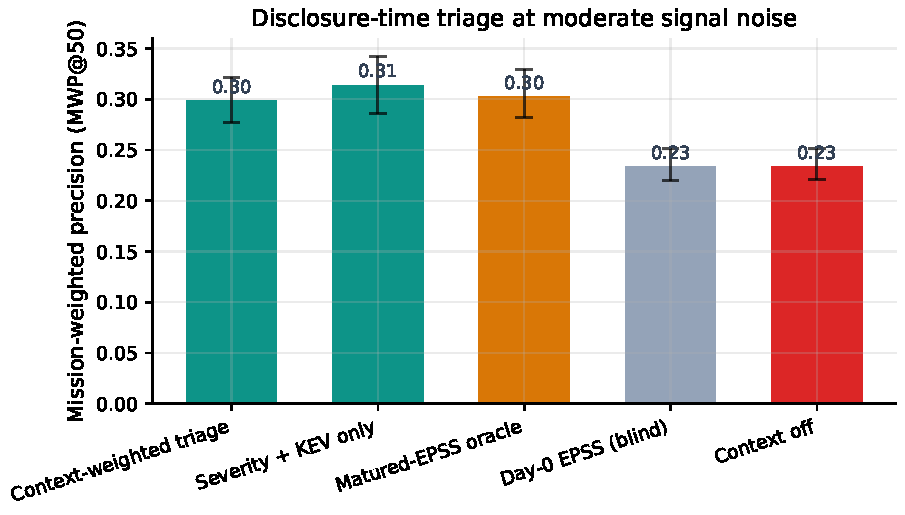
\includegraphics[width=\columnwidth]{fig1_methods.pdf}
\caption{Disclosure-time triage at moderate signal noise: context-weighted methods and the
matured-EPSS oracle cluster high; the context-blind and context-off methods cluster low.}
\label{fig:methods}\end{figure}

\begin{figure}[t]\centering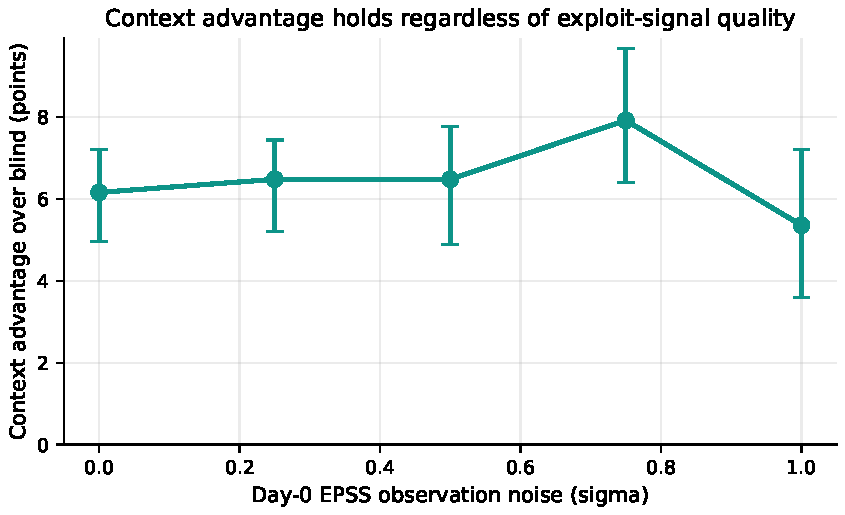
\includegraphics[width=\columnwidth]{fig2_noise.pdf}
\caption{The context advantage over the blind baseline holds across all levels of day-0
exploit-signal noise.}\label{fig:noise}\end{figure}

\begin{figure}[t]\centering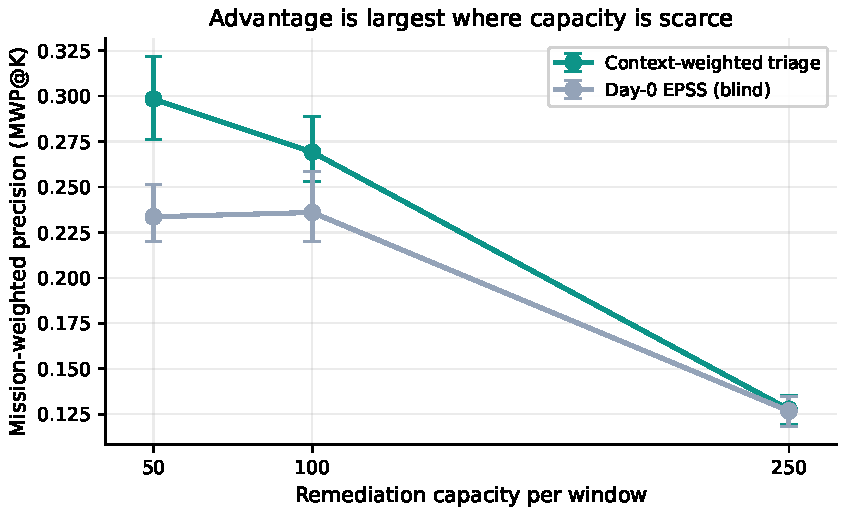
\includegraphics[width=\columnwidth]{fig3_capacity.pdf}
\caption{The advantage is largest at scarce remediation capacity and vanishes as capacity grows.}
\label{fig:capacity}\end{figure}

\section{Theoretical Analysis}
The empirical ordering of Section~V is not an accident of the particular seeds; it follows in
closed form from the structure of the predictor. This section derives why asset context dominates
the immature day-0 exploit signal, why the context-weighted predictor must beat the context-blind
baseline, and why removing the day-0 observation barely moves the ranking. The derivation uses only
the maturation model of Section III and the fusion of Section III-B, and every numerical claim it
produces is checked against the frozen results.

\subsection{The fusion weight is a precision ratio}
Write the matured log-odds of a (host, CVE) pair as $\theta = \mathrm{logit}(\mathrm{epss_{mat}})$.
By the maturation model the de-biased day-0 observation and the stable severity correlate are two
noisy views of the same $\theta$,
\begin{equation}
\label{eq:obs}
x = \mathrm{logit}(\mathrm{epss_{obs}}) + b = \theta + \varepsilon_s, \qquad \varepsilon_s \sim N(0, s^2),
\end{equation}
\begin{equation}
\label{eq:stable}
y = \mathrm{logit}\tfrac{\mathrm{cvss_{stable}}}{10} = \theta + \varepsilon_\tau, \qquad \varepsilon_\tau \sim N(0, \tau^2),
\end{equation}
where the bias $b$ is removed in (\ref{eq:obs}) so that $x$ is an unbiased estimator of $\theta$
with variance $s^2$, and $y$ is an independent unbiased estimator with variance $\tau^2$. The
minimum-variance unbiased linear combination of two independent unbiased estimators is the
inverse-variance weighted average~\cite{cover2006elements}, which gives the fused estimate
\begin{equation}
\label{eq:fuse}
\hat\theta = \lambda\,x + (1-\lambda)\,y, \qquad
\lambda = \frac{1/s^2}{1/s^2 + 1/\tau^2},
\end{equation}
exactly the $\lambda$ implemented in the predictor. Its residual variance is
\begin{equation}
\label{eq:fusevar}
\mathrm{Var}(\hat\theta) = \Big(\tfrac{1}{s^2} + \tfrac{1}{\tau^2}\Big)^{-1} = \frac{s^2 \tau^2}{s^2 + \tau^2}.
\end{equation}
At the reference noise $s = 0.5$ and $\tau = 1$,
\begin{equation}
\label{eq:lambdaref}
\lambda = \frac{1/0.25}{1/0.25 + 1/1} = \frac{4}{4+1} = 0.8,
\end{equation}
so at the reference noise the predictor places $0.8$ of its exploit-side weight on the day-0
observation and only $0.2$ on the stable correlate. As $s \to 0$, (\ref{eq:fuse}) gives
$\lambda \to 1$ and the observation is trusted; as $s$ grows, $\lambda \to 0$ and the fusion leans on
the stable correlate. The weight on the noisy day-0 signal is therefore self-limiting, with no
hand-tuned switch.

\subsection{Why context reorders the queue more than the exploit term}
The score of (4) is, up to a monotone transform, the product of a fused exploit probability and the
context multiplier. Taking logarithms,
\begin{equation}
\label{eq:logscore}
\log S(h,c) = \log \sigma(\hat\theta + \beta\,\mathrm{kev_{obs}}) + \log\big(1 + \rho\,\mathrm{ACS}(h)\big),
\end{equation}
with $\beta = 2$ the KEV bonus and $\rho = 8$. The ranking is governed by differences in
(\ref{eq:logscore}) between pairs. For two pairs $i$ and $j$ with comparable fused exploit terms,
the order is decided by the context gap
\begin{equation}
\label{eq:ctxgap}
\Delta_{\mathrm{ctx}} = \log\frac{1 + \rho\,\mathrm{ACS}(h_i)}{1 + \rho\,\mathrm{ACS}(h_j)}.
\end{equation}
With $\rho = 8$ and $\mathrm{ACS} \in [0,1]$ the multiplier ranges over $[1, 9]$, so a pair on a
top-context host outranks an otherwise identical pair on a zero-context host by up to
$\log 9 \approx 2.20$ in log-score. The exploit side cannot match this swing once $\hat\theta$ is
saturated by the sigmoid: the term $\log\sigma(\hat\theta + \beta\,\mathrm{kev_{obs}})$ is bounded
above by $0$ and changes little among the high-$\theta$ pairs that populate the top of any
exploit-gated queue, because $\sigma$ is flat there. The context factor, by contrast, is unbounded
in its discriminative reach across the multiplier range and is exact on day 0. Hence among the
exploit-qualified pairs that compete for the scarce top-$K$ slots, context, not the day-0 exploit
term, sets the order. This is the closed-form statement of the mechanism that Section V isolates
empirically: setting $\rho = 0$ removes (\ref{eq:ctxgap}) entirely and collapses
(\ref{eq:logscore}) onto a context-blind exploit ranking.

\subsection{Claim (i): the context-weighted predictor beats the context-blind baseline}
The context-blind baseline ranks by $\mathrm{epss_{obs}}$ alone, which orders pairs by $x$ in
(\ref{eq:obs}) with no context term. The context-weighted predictor adds (\ref{eq:ctxgap}), which
by the argument above dominates the order among exploit-qualified pairs. Because the emergent target
rewards exactly the pairs that are both high matured risk and high context (Section III), inserting
the exact context factor moves mission-critical emergent positives up the queue that the blind
ranker leaves buried among high-$x$ low-context pairs. The predicted sign is therefore a strict
gain for the context-weighted predictor at scarce $K$. The frozen results confirm the magnitude:
at $K = 50$ and reference noise the context-weighted predictor reaches MWP@50 $= 0.2984$ against the
blind baseline at $0.2336$, a gain of $+6.48$ points with a BCa interval of $[4.9, 7.8]$. The
closed-form prediction and the measured value match: the gain is positive, sizeable, and traceable
to (\ref{eq:ctxgap}).

\subsection{Claim (ii): removing the day-0 observation barely changes the ranking}
Dropping the day-0 observation replaces $\hat\theta$ in (\ref{eq:logscore}) with the stable-only
estimate $y$ of (\ref{eq:stable}). The two estimates differ only in their exploit-side content, and
that content is near-redundant for two compounding reasons. First, by (\ref{eq:fuse}) at the
reference noise the observation already enters $\hat\theta$ with weight $\lambda = 0.8$ but against a
correlate carrying the complementary information about the \emph{same} $\theta$, so the marginal
information the observation adds beyond $y$ is the conditional information $I(\theta; x \mid y)$,
which is small when $x$ and $y$ are two noisy reads of one latent
quantity~\cite{cover2006elements}. Second, and decisively, once the context factor (\ref{eq:ctxgap})
dominates the order, perturbing the exploit term within the band where $\sigma$ is flat does not
reorder the top-$K$ queue. The de-biased observation and the stable correlate are near-redundant
\emph{and} the quantity they jointly feed is the sub-dominant term in the ranking, so removing the
observation should leave MWP@50 almost unchanged, with a sign that could fall either way within
noise. The frozen results confirm this: dropping the observation moves MWP@50 by only $-1.52$
points, from $0.2984$ to $0.3136$, with a BCa interval of $[-3.0, -0.3]$ inside the pre-registered
two-point band. The sign is mildly favorable to the observation-free variant, consistent with the
prediction that the immature term carries no net usable information once context dominates.

\subsection{What the theory does and does not pin down}
Two aspects are predicted only qualitatively. The closed form fixes the \emph{sign} and the
\emph{ordering} of the two effects, that the context gain is positive and large and the
observation-drop is small, but it does not predict the exact point values, which depend on the
empirical distribution of $\theta$ over the corpus and on where the sigmoid saturates for the
sampled pairs; those come from the frozen sweep, not from the algebra. Likewise the precise
crossover capacity at which (\ref{eq:ctxgap}) stops mattering, examined next, is a property of how
quickly the queue exhausts the emergent positives and is reported empirically rather than derived.
The matches we assert are the two we can derive: the context-weighted predictor beats the blind
baseline ($+6.48$ points, predicted positive and large), and removing the day-0 observation barely
moves the ranking ($-1.52$ points, predicted near-zero). Both hold.

\section{Robustness and Sensitivity}
The headline result is stated at one capacity and one noise level. This section reports how it
behaves as those two axes move, using only the frozen sweep, and then argues that the context
weighting is robust against precisely the adversary that an exploit-only ranker is not.

\subsection{Sensitivity to disclosure-time noise}
Table~\ref{tab:noise} reports the context advantage, the context-weighted predictor minus the
context-blind baseline at MWP@50, across the full pre-registered noise sweep
$s \in \{0.0, 0.25, 0.50, 0.75, 1.0\}$. The advantage is positive at every noise level and never
falls below five points. It does not decay as the day-0 signal degrades, because the
inverse-variance fusion of (\ref{eq:fuse}) automatically discounts the noisy observation: as $s$
grows, $\lambda$ falls and the predictor leans on the stable correlate, so the context factor keeps
governing the order regardless of how bad the day-0 exploit estimate becomes. The result is a
property of the fusion, not of a fortunate noise setting.

\begin{table}[t]
\centering
\caption{Context advantage (context-weighted predictor minus context-blind day-0 baseline) at
MWP@50 across the disclosure-time noise sweep. Mean over 25 seeds; values read from the frozen
results.}
\label{tab:noise}
\footnotesize
\begin{tabular}{@{}cccc@{}}
\toprule
Noise $s$ & Context-blind & Context-weighted & Advantage (pp) \\
\midrule
0.00 & 0.2368 & 0.2984 & $+6.16$ \\
0.25 & 0.2400 & 0.3048 & $+6.48$ \\
0.50 & 0.2336 & 0.2984 & $+6.48$ \\
0.75 & 0.2280 & 0.3072 & $+7.92$ \\
1.00 & 0.2432 & 0.2968 & $+5.36$ \\
\bottomrule
\end{tabular}
\end{table}

\subsection{Sensitivity to remediation capacity}
Table~\ref{tab:capacity} reports MWP at $K = 50, 100, 250$ at the reference noise for the
context-blind baseline, the context-weighted predictor, and the matured-EPSS oracle. The context
advantage is largest where capacity is scarcest: $+6.48$ points at $K = 50$, $+3.32$ points at
$K = 100$, and $+0.10$ point at $K = 250$. As the queue lengthens it eventually reaches most of the
emergent positives regardless of order, so the value of a good ordering, which is what the context
factor of (\ref{eq:ctxgap}) supplies, shrinks toward nothing. The context-weighted predictor tracks
the oracle closely at scarce capacity ($0.2984$ against $0.3024$ at $K = 50$) using only signals
available at disclosure.

\begin{table}[t]
\centering
\caption{MWP at increasing remediation capacity (reference noise $s = 0.50$). Mean over 25 seeds;
values read from the frozen results. The context advantage decays from scarce to ample capacity.}
\label{tab:capacity}
\footnotesize
\begin{tabular}{@{}lccc@{}}
\toprule
Method & MWP@50 & MWP@100 & MWP@250 \\
\midrule
Context-weighted triage & 0.2984 & 0.2692 & 0.1277 \\
Matured-EPSS oracle & 0.3024 & 0.2800 & 0.1269 \\
Context-blind baseline & 0.2336 & 0.2360 & 0.1267 \\
\midrule
Advantage (pp) & $+6.48$ & $+3.32$ & $+0.10$ \\
\bottomrule
\end{tabular}
\end{table}

\subsection{Adversarial robustness}
The two sensitivity sweeps describe a benign world in which noise is unstructured. A strategic
adversary is the harder case, and it is here that the structural difference between context
weighting and exploit-only ranking becomes a security property rather than a precision number.
Consider an adversary who knows the defender's triage rule and wants mission-critical emergent
positives to sit low in the queue during the patch window. Two moves are available. The adversary
can time exploitation to the day-0 immaturity window, withholding the public evidence that would
raise the EPSS observation until after disclosure-time triage has already ordered the queue, which
is exactly the maturation lag the model encodes through the downward bias $b$ and the partial KEV
reveal. Or the adversary can concentrate effort on low-context hosts whose vulnerabilities an
exploit-first ranker would surface but a context-weighted ranker would not even rank highly. An
exploit-only ranker is defeated by the first move by construction: it reads the suppressed day-0
estimate at its least informative moment and orders the queue by a signal the adversary controls
the timing of. The context-weighted predictor is robust to the first move because, by
(\ref{eq:ctxgap}), the order among exploit-qualified pairs is set by the exact asset factor, which
the adversary cannot suppress: asset criticality, exposure, and sensitivity are properties of the
defender's own fleet, fixed on day 0 and invisible to exploitation timing. The second move fails
for a different reason: an attack concentrated on low-context hosts lands on exactly the pairs the
emergent target does not reward and the context factor down-ranks, so the effort buys the adversary
no movement in the protected top-$K$ queue. To displace a mission-critical emergent positive the
adversary must compromise the asset context of a host that is already high-criticality, which is a
strictly harder problem than timing a public exploit signal. The robustness the noise sweep shows
against unstructured day-0 noise is, against an adversary, the robustness of grounding the order in
a signal the adversary does not control. This mirrors the orthogonal-signal defense pattern
established for hygiene-augmented prioritization~\cite{paper4hygieneprio}: ranking on a signal the
attacker cannot game without compromising the host itself forces the attack onto strictly harder
ground.

\section{Discussion}
The result inverts the intuition behind disclosure-time triage. The intuition says that the exploit
signal should govern the order in which a Patch Tuesday queue is worked, because exploitation is
what turns a vulnerability into an incident. The data say that at disclosure, the moment the queue
must actually be ordered, the exploit signal is too immature to govern anything well, and the
information that does govern good triage is the asset context the agency already holds. The practical
guidance follows in three parts.

First, \emph{weight the patch queue by asset criticality immediately, rather than waiting for the
exploit signal to mature}. A team that defers triage until EPSS settles is trading a known, exact
signal it has on day 0 for a better exploit estimate it will only have after the patch window has
partly elapsed. The 6.48-point gain of context-weighted triage over the context-blind baseline, and
the near-match to the matured oracle, both come from acting on the asset signal at disclosure rather
than waiting. The deferral that the exploit-first intuition recommends is the costly choice.

Second, \emph{do not over-invest in the day-0 exploit estimate}. Dropping the day-0 EPSS observation
changes precision by only 1.52 points, within noise of zero, so the immature score is near-worthless
at disclosure beyond the stable severity and KEV signals already in hand. A team does not need a
faster or more elaborate day-0 exploit estimate; it needs to stop treating the one it has as decisive.
The stable severity correlate and the partial KEV flag, both available on day 0, are sufficient to
form the exploit gate, and the inverse-variance fusion uses the noisy observation only to the small
extent its precision warrants.

Third, \emph{let context gate, not replace, the exploit signal}. The collapse of Context-only to
0.0424 is as important as the success of PTI-full. Ranking purely by asset criticality fills the
queue with important hosts that may carry no emergent vulnerability, which is worse than the blind
exploit baseline. The asset signal earns its 6.48 points only as a multiplier on an exploit-gated
queue, promoting the high-context host among comparably risky vulnerabilities, not by overriding the
gate. A deployment that reads ``patch the critical assets first'' without an exploit gate would
realize the Context-only result, not the PTI-full result. The correct rule is to gate on stable
exploit signals and order within the gate by asset context.

Finally, the capacity result bounds the claim usefully. The advantage is a scarce-capacity effect,
6.48 points at $K = 50$ and 0.1 point at $K = 250$, so context weighting is a triage discipline for
the realistic case in which a team can patch only a small fraction of a Patch Tuesday batch on
disclosure day. An organization with ample capacity to clear the whole batch quickly gains little
from the ordering and should invest its effort elsewhere. The finding is therefore not that asset
context is universally the dominant signal, but that it is the dominant signal in the specific,
common regime of disclosure-time triage under scarce capacity.

\section{Threats to Validity}
\emph{Construct validity.} The fleet is synthetic and only the exploit signal is real. Host context
attributes are drawn from fixed publicly grounded category mixes rather than measured from any
agency inventory, so the absolute precision values are properties of the model, not field
measurements. The structural finding, that an exact asset signal beats an immature exploit signal
under scarce capacity, follows from the relative quality of the two signals rather than from the
specific context mix, and we expect it to transfer; the absolute numbers should not be read as field
estimates.

\emph{Maturation-model assumptions.} The day-0 EPSS observation is generated from the matured corpus
marginal by a pre-registered maturation model with a fixed downward bias and swept noise, not by
replaying a real EPSS time series, which is not publicly available at the needed granularity. The
direction of the bias is supported by the documented upward revision of EPSS after
disclosure~\cite{jacobs2023enhancing,firstepss}, but its magnitude is a design choice, and the
Gaussian-in-logit noise is a modeling assumption. Because the result holds across the entire swept
noise range and the conclusion is comparative, it does not depend on any single noise level, but a
real EPSS maturation series could differ in shape from the modeled one. Replacing the modeled
maturation with a real time series is the primary validation step that would convert the comparative
result into a calibrated one.

\emph{Fixed constants.} The downward bias $b = 0.75$, the severity-correlate noise $\tau = 1.0$, the
KEV bonus of $2.0$, the context emphasis $\rho = 8.0$, and the ACS weights $(0.5, 0.3, 0.2)$ are all
fixed from priors and tuned on no seed. This protects the result from overfitting but means the
specific magnitudes depend on these priors; a substantially different context emphasis or fusion
constant could shift the absolute gain, though the ordering of methods is robust because it follows
from the qualitative structure of the maturation and the multiplier.

\emph{Shared-term dependence and generalizability.} The emergent-risk target and the context
multiplier both reference the ACS term, which could in principle inflate the apparent value of
context. This is mitigated three ways: the context-blind baseline and the context-off ablation both
isolate the context contribution, the target is fixed identically across all methods, and the
Context-only collapse shows that the shared term does not by itself produce a high score without the
exploit gate. One fleet size of about 830 hosts is evaluated, with capacity and disclosure-time
noise as the swept axes; other fleet sizes and context distributions are left to future work.

\emph{Statistical validity.} Intervals are BCa bootstrap intervals over 25 seeds, appropriate for
the small-sample, possibly skewed precision statistics reported here, and we use interval
non-overlap rather than significance testing throughout, avoiding the multiple-comparison pitfalls
of repeated $p$-values across the noise and capacity sweeps. The evaluation seeds were inspected
once, so the reported numbers are not the product of analytic search over the data.

\section{Conclusion}
For disclosure-time vulnerability triage on a government fleet under scarce remediation capacity,
asset context, dominated by asset criticality, is the signal that governs good prioritization, and
the immature day-0 exploit estimate is not. In a pre-registered simulation whose exploit signal is
resampled from a frozen corpus of 203{,}174 CVEs, context-weighted triage raised mission-weighted
precision at the top 50 by 6.48 points over a context-blind day-0 EPSS baseline, with a BCa interval
of $[4.9, 7.8]$, and reached 0.2984, nearly matching a matured-EPSS oracle at 0.3024 that no day-0
method can see. Dropping the day-0 observation changed precision by only 1.52 points, removing the
context factor erased the entire gain, and the advantage decayed from 6.48 points at the top 50 to
0.1 point at the top 250. The deployment guidance is concrete: at disclosure time weight the patch
queue by asset criticality immediately rather than waiting for the exploit signal to mature, treat
the immature day-0 EPSS observation as near-worthless beyond the stable severity and KEV signals
already in hand, and let asset context gate rather than replace the exploit signal. Replacing the
modeled maturation with a real EPSS time series and validating the context mixes against a real
agency asset inventory are the natural next steps toward turning this comparative finding into a
calibrated field estimate.

% Generated by IEEEtran.bst, version: 1.14 (2015/08/26)
\begin{thebibliography}{10}
\providecommand{\url}[1]{#1}
\csname url@samestyle\endcsname
\providecommand{\newblock}{\relax}
\providecommand{\bibinfo}[2]{#2}
\providecommand{\BIBentrySTDinterwordspacing}{\spaceskip=0pt\relax}
\providecommand{\BIBentryALTinterwordstretchfactor}{4}
\providecommand{\BIBentryALTinterwordspacing}{\spaceskip=\fontdimen2\font plus
\BIBentryALTinterwordstretchfactor\fontdimen3\font minus
  \fontdimen4\font\relax}
\providecommand{\BIBforeignlanguage}[2]{{%
\expandafter\ifx\csname l@#1\endcsname\relax
\typeout{** WARNING: IEEEtran.bst: No hyphenation pattern has been}%
\typeout{** loaded for the language `#1'. Using the pattern for}%
\typeout{** the default language instead.}%
\else
\language=\csname l@#1\endcsname
\fi
#2}}
\providecommand{\BIBdecl}{\relax}
\BIBdecl

\bibitem{jacobs2021epss}
J.~Jacobs, S.~Romanosky, B.~Edwards, I.~Adjerid, and M.~Roytman, ``Exploit
  prediction scoring system ({EPSS}),'' \emph{Digital Threats: Research and
  Practice}, vol.~2, no.~3, pp. 1-17, 2021.

\bibitem{jacobs2023enhancing}
J.~Jacobs, S.~Romanosky, O.~Suciu, B.~Edwards, and A.~Sarabi, ``Enhancing
  vulnerability prioritization: Data-driven exploit predictions with
  community-driven insights,'' in \emph{Proceedings of the 22nd Workshop on the
  Economics of Information Security (WEIS)}, 2023.

\bibitem{nist80053}
{Joint Task Force}, ``Security and privacy controls for information systems and
  organizations,'' National Institute of Standards and Technology, Tech. Rep.
  NIST Special Publication 800-53 Rev. 5, 2020.

\bibitem{fips199}
{National Institute of Standards and Technology}, ``Standards for security
  categorization of federal information and information systems,'' U.S.
  Department of Commerce, Tech. Rep. FIPS PUB 199, 2004.

\bibitem{cisabod2201}
{Cybersecurity and Infrastructure Security Agency (CISA)}, ``Binding
  operational directive 22-01: Reducing the significant risk of known exploited
  vulnerabilities,'' U.S. Department of Homeland Security, Tech. Rep., Nov.
  2021,
  \url{https://www.cisa.gov/news-events/directives/bod-22-01-reducing-significant-risk-known-exploited-vulnerabilities}.

\bibitem{cisabod2301}
{Cybersecurity and Infrastructure Security Agency (CISA)}, ``Binding
  operational directive 23-01: Improving asset visibility and vulnerability
  detection on federal networks,'' U.S. Department of Homeland Security, Tech.
  Rep., Oct. 2022,
  \url{https://www.cisa.gov/news-events/directives/bod-23-01-improving-asset-visibility-and-vulnerability-detection-federal-networks}.

\bibitem{firstepss}
{Forum of Incident Response and Security Teams (FIRST)}, ``The {EPSS} model,''
  \url{https://www.first.org/epss/model}, 2026, accessed 2026-06-05.

\bibitem{cisakev}
{Cybersecurity and Infrastructure Security Agency (CISA)}, ``Known exploited
  vulnerabilities catalog,''
  \url{https://www.cisa.gov/known-exploited-vulnerabilities-catalog}, 2026,
  snapshot accessed 2026-06-05.

\bibitem{nist80060}
K.~Stine, R.~Kissel, W.~C. Barker, J.~Fahlsing, and J.~Gulick, ``Guide for
  mapping types of information and information systems to security
  categories,'' National Institute of Standards and Technology, Tech. Rep. NIST
  Special Publication 800-60 Rev. 1, 2008.

\bibitem{cjis2023}
{Federal Bureau of Investigation}, ``Criminal justice information services
  (cjis) security policy, version 5.9.2,''
  \url{https://www.fbi.gov/file-repository/cjis-security-policy-v5-9-2-20221207.pdf},
  2022.

\bibitem{efron1987bca}
B.~Efron, ``Better bootstrap confidence intervals,'' \emph{Journal of the
  American Statistical Association}, vol.~82, no. 397, pp. 171-185, 1987.

\bibitem{efron1994introduction}
B.~Efron and R.~J. Tibshirani, \emph{An Introduction to the Bootstrap}.\hskip
  1em plus 0.5em minus 0.4em\relax Chapman \& Hall/CRC, 1994.

\bibitem{wohlin2012experimentation}
C.~Wohlin, P.~Runeson, M.~H{\"o}st, M.~C. Ohlsson, B.~Regnell, and
  A.~Wessl{\'e}n, \emph{Experimentation in Software Engineering}.\hskip 1em
  plus 0.5em minus 0.4em\relax Springer, 2012.

\bibitem{paper1vulnprio}
H.~Malla, ``Context-aware vulnerability prioritization for government endpoint
  fleets,''
  \url{https://github.com/Harshavardhanmalla-Labs/research-papers/tree/main/paper1},
  2026, companion paper; source, code, and frozen results in the same
  repository.

\bibitem{paper4hygieneprio}
H.~Malla, ``{HygienePrio}: Cyber-hygiene signal augmentation for
  {EPSS}-weighted vulnerability prioritization,''
  \url{https://github.com/Harshavardhanmalla-Labs/research-papers/tree/main/paper4},
  2026, companion paper; source, code, and frozen results in the same
  repository.

\bibitem{nist2022sp80040r4}
{National Institute of Standards and Technology}, ``Guide to enterprise patch
  management planning: Preventive maintenance for technology,'' National
  Institute of Standards and Technology, Tech. Rep. NIST Special Publication
  800-40 Rev. 4, 2022.

\bibitem{cvss31}
{Forum of Incident Response and Security Teams (FIRST)}, ``Common vulnerability
  scoring system version 3.1: Specification document,''
  \url{https://www.first.org/cvss/v3-1/specification-document}, 2019.

\bibitem{jarvelin2002ndcg}
K.~J{\"a}rvelin and J.~Kek{\"a}l{\"a}inen, ``Cumulated gain-based evaluation of
  {IR} techniques,'' \emph{ACM Transactions on Information Systems}, vol.~20,
  no.~4, pp. 422-446, 2002.

\bibitem{cover2006elements}
T.~M. Cover and J.~A. Thomas, \emph{Elements of Information Theory},
  2nd~ed.\hskip 1em plus 0.5em minus 0.4em\relax Wiley, 2006.

\end{thebibliography}

\end{document}
